\section{Voltage Mode Buck Converter}
Het schema in \autoref{fig:Schematic} is opgebouwd in dit hoofdstuk. Dit is een voltage mode buck converter. De breadboard opstelling, volgens het schema, is te zien in \autoref{fig:breadboard_opstelling}. 

Met 15V over \(V_{in}\) , krijgen we een output van ongeveer 5V (Buck converter). De input settling ripple is te zien in \autoref{fig:Scope1}, \autoref{fig:Scope2} en \autoref{fig:Scope3}. 

\begin{figure}[b]
    \centering
    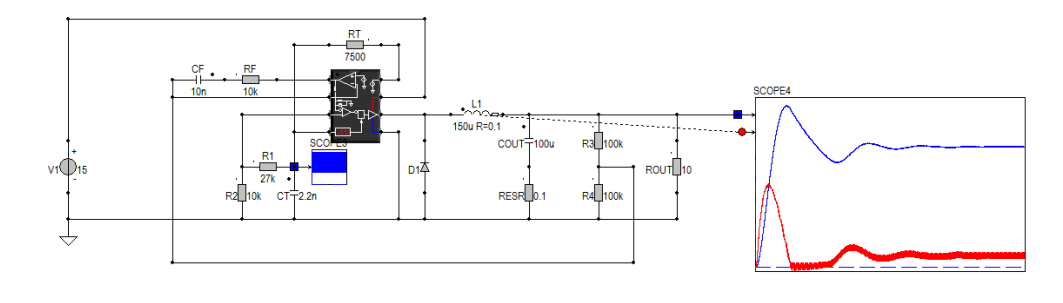
\includegraphics[width=0.8\linewidth]{img/hfd4/Schematic.png}
    \caption{Schematic}
    \label{fig:Schematic}
\end{figure}


\begin{figure}[h!]
    \centering
    \begin{subfigure}[b]{0.45\linewidth}
        \centering
        \includegraphics[width=\linewidth]{img/hfd4/Breadboard 1.png}
        \caption{Breadboard opstelling foto 1}
        \label{fig:Breadboard 1}
    \end{subfigure}%
    \hfill
    \begin{subfigure}[b]{0.45\linewidth}
        \centering
        \includegraphics[angle=90, width=\linewidth]{img/hfd4/Breadboard 2.png}
        \caption{Breadboard opstelling foto 1}
        \label{fig:Breadboard 2}
    \end{subfigure}
    
    \caption{Breadboard opstellingen}
    \label{fig:breadboard_opstelling}
\end{figure}

\begin{figure}[b]
    \centering
    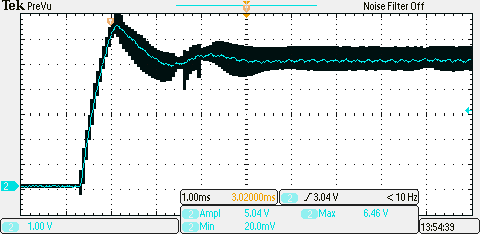
\includegraphics[width=0.6\linewidth]{img/hfd4/Scope/TEK00002.PNG}
    \caption{Scope1}
    \label{fig:Scope1}
\end{figure}

\begin{figure}[b]
    \centering
    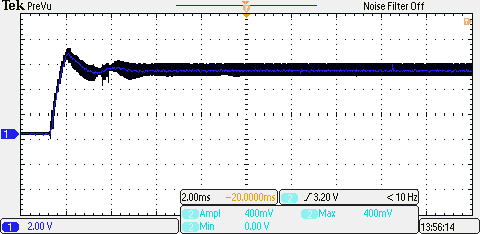
\includegraphics[width=0.6\linewidth]{img/hfd4/Scope/TEK00003.PNG}
    \caption{Scope2}
    \label{fig:Scope2}
\end{figure}

\begin{figure}[b]
    \centering
    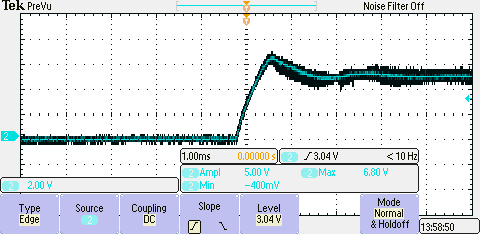
\includegraphics[width=0.6\linewidth]{img/hfd4/Scope/TEK00004.PNG}
    \caption{Scope3}
    \label{fig:Scope3}
\end{figure}
